\section{Mức độ 5,6 điểm}
\Opensolutionfile{ans}[ans/CD5/Muc_5_6]
\begin{dang}{Nhận dạng hàm số thường gặp thông qua đồ thị}
\end{dang}
\begin{ex}%[2D1Y5-1]
	[Đề Minh Họa 2020 Lần 1]
	\immini{
		Đồ thị của hàm số nào dưới đây có dạng như đường cong trong dưới đây?
		\choice
		{\True $ y=-x^4+2x^2$}
		{$ y=x^4-2x^2$}
		{$ y=x^3-3x^2$}
		{$ y=-x^3+3x^2$}
	}{
		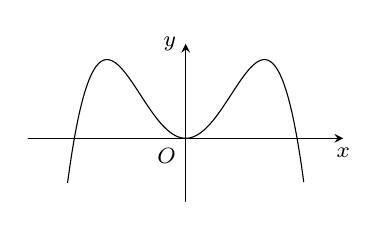
\begin{tikzpicture}[line cap=round, line join=round, font=\footnotesize, >=stealth, scale=1]
			\tikzset{label style/.style={font=\footnotesize}}
			\draw[->] (-2,0)--(2,0) node[below]{$x$};
			\draw[->] (0,-0.8)--(0,1.2) node[left]{$y$};
			\draw[smooth, samples=100] plot[domain=-1.5:1.5] (\x, {-(\x)^4+2*(\x)^2});
			\node at (0,0)[below left]{$O$};
		\end{tikzpicture}	
	}
	\loigiai{
		Từ hình dạng của đồ thị ta loại phương án $ y=x^3-3x^2$.\\
		Nhận thấy $\lim\limits_{x\to\pm\infty}f(x)=-\infty $ suy ra hệ số của $x^4$ âm nên chọn phương án $ y=-x^4+2x^2$.}
\end{ex}

\begin{ex}%[2D1Y5-1]
	[Đề Tham Khảo 2020 Lần 2]
	\immini{
		Đồ thị của hàm số nào dưới đây có dạng như đường cong trong hình bên?
		\choice
		{\True $ y=x^3-3x$}
		{$ y=-x^3+3x$}
		{$ y=x^4-2x^2$}
		{$ y=-x^4+2x^2$}
	}{
		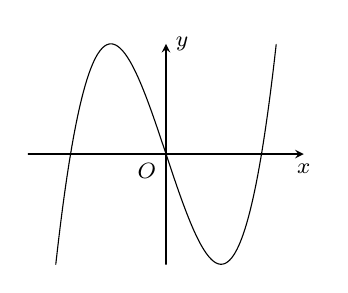
\begin{tikzpicture}[line cap=round, line join=round, font=\footnotesize, >=stealth, scale=0.7]
			\tikzset{label style/.style={font=\footnotesize}}
			\draw[->] (-2.5,0)--(2.5,0) node[below]{$x$};
			\draw[->] (0,-2)--(0,2) node[right]{$y$};
			\draw[smooth, samples=100] plot[domain=-2:2] (\x, {(\x)^3-3*(\x)});
			\node at (0,0)[below left]{$O$};
		\end{tikzpicture}			
	}
	\loigiai{
		Đường cong có dạng của đồ thị hàm số bậc $3$ với hệ số $a>0$ nên chỉ có hàm số $y=x^3-3x$ thỏa yêu cầu bài toán.
	}
\end{ex}	

\begin{ex}%[2D1Y5-1]
	[Mã 101 - 2020 Lần 1]
	\immini{
		Đồ thị hàm số nào dưới đây có dạng như đường cong trong hình bên?
		\choice
		{$ y=x^3-3x^2+1$}
		{$ y=-x^3+3x^2+1$}
		{\True $ y=-x^4+2x^2+1$}
		{$ y=x^4-2x^2+1$}
	}{
		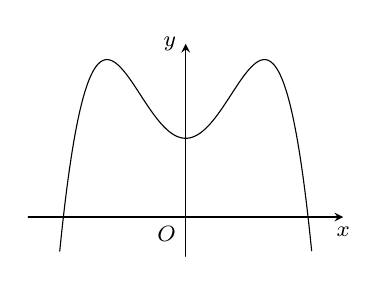
\begin{tikzpicture}[line cap=round, line join=round, font=\footnotesize, >=stealth, scale=1]
			\tikzset{label style/.style={font=\footnotesize}}
			\draw[->] (-2,0)--(2,0) node[below]{$x$};
			\draw[->] (0,-0.5)--(0,2.2) node[left]{$y$};
			\draw[smooth, samples=100] plot[domain=-1.6:1.6] (\x, {-(\x)^4+2*(\x)^2+1});
			\node at (0,0)[below left]{$O$};
		\end{tikzpicture}
	}
	\loigiai{
		Từ hình có đây là hình dạng của đồ thị hàm bậc $4$.\\
		$\lim\limits_{x\to-\infty} f(x)= \lim\limits_{x\to+\infty} f(x)=-\infty\Rightarrow a<0$.}
\end{ex}	

\begin{ex}%[2D1Y5-1]
	[Mã 102 - 2020 Lần 1]
	\immini{
		Đồ thị hàm số nào dưới đây có dạng như đường cong trong hình bên?
		\choice
		{\True $y-x^4+2x^2$}
		{$y=-x^3+3x$}
		{$y=x^4-2x^2$}
		{$y=x^3-3x$}
	}{
		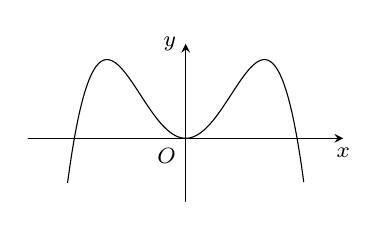
\begin{tikzpicture}[line cap=round, line join=round, font=\footnotesize, >=stealth, scale=1]
			\tikzset{label style/.style={font=\footnotesize}}
			\draw[->] (-2,0)--(2,0) node[below]{$x$};
			\draw[->] (0,-0.8)--(0,1.2) node[left]{$y$};
			\draw[smooth, samples=100] plot[domain=-1.5:1.5] (\x, {-(\x)^4+2*(\x)^2});
			\node at (0,0)[below left]{$O$}; 
		\end{tikzpicture}
	}
	\loigiai{
		Đồ thị trong hình là đồ thị hàm $y=ax^4+bx^2+c$ với $a<0$.
	}
\end{ex}	

\begin{ex}%[2D1Y5-1]
	[Mã 103 - 2020 Lần 1]
	\immini{
		Cho hàm số bậc ba $y=f(x)$ có đồ thị là đường cong trong hình bên. Số nghiệm thực của phương trình $f(x)=1$ là
		\choice
		{$1$}
		{$0$}
		{$2$}
		{\True $3$}
	}{
		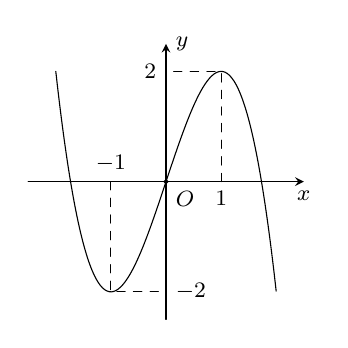
\begin{tikzpicture}[line cap=round, line join=round, font=\footnotesize, >=stealth, scale=0.7]
			\tikzset{label style/.style={font=\footnotesize}}
			\draw[->] (-2.5,0)--(2.5,0) node[below]{$x$};
			\draw[->] (0,-2.5)--(0,2.5) node[right]{$y$};
			\draw[smooth, samples=100] plot[domain=-2:2] (\x, {-(\x)^3+3*(\x)});
			\draw[dashed] (-1,0) node[above]{$-1$}--(-1,-2)--(0,-2)node[right]{$-2$}
			(1,0) node[below]{$1$}--(1,2)--(0,2) node[left]{$2$};
			\draw[fill=black] (0,0) circle (1pt) node[below right]{$O$};			
		\end{tikzpicture}
	}
	\loigiai{
		Từ đồ thị hàm số ta có số nghiệm thực của phương trình $f(x)=1$ là $3$ .}
\end{ex}	

\begin{ex}%[2D1Y5-1]
	[Mã 104 - 2020 Lần 1]
	\immini{
		Đồ thị hàm số nào dưới đây có dạng như đường cong trong hình bên?
		\choice
		{\True $ y=x^4-2x^2+1$}
		{$ y=-x^3+3x^2+1$}
		{$ y=x^3-3x^2+1$}
		{$ y=-x^4+2x^2+1$}
	}{
		\begin{tikzpicture}[line cap=round, line join=round, font=\footnotesize, >=stealth, scale=1]
			\tikzset{label style/.style={font=\footnotesize}}
			\draw[->] (-2,0)--(2,0) node[below]{$x$};
			\draw[->] (0,-0.6)--(0,2) node[left]{$y$};
			\draw[smooth, samples=100] plot[domain=-1.5:1.5] (\x, {(\x)^4-2*(\x)^2+1});
			\node at (0,0)[below left]{$O$}; 
		\end{tikzpicture}
	}
	\loigiai{
		Dựa vào hình vẽ, ta thấy đồ thị hàm số có ba điểm cực trị nên loại các phương án $y=-x^3+3x^2+1$ và $ y=x^3-3x^2+1$.\\
		Mặt khác, ta thấy $\lim\limits_{x\to+\infty} \left(x^4-2x^2+1\right)=+\infty $ nên chọn đáp án $ y=x^4-2x^2+1$.}
\end{ex}	

\begin{ex}%[2D1Y5-1]
	[Mã 101 - 2020 Lần 2]
	\immini{
		Đồ thị hàm số nào dưới đây có dạng như đường cong hình bên
		\choice
		{$ y=x^4-2x^2-2$}
		{\True $ y=-x^3+3x^2-2$}
		{$ y=x^3-3x^2-2$}
		{$ y=-x^4+2x^2-2$}
	}{
		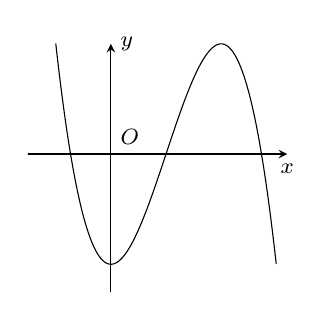
\begin{tikzpicture}[line cap=round, line join=round, font=\footnotesize, >=stealth, scale=0.7]
			\tikzset{label style/.style={font=\footnotesize}}
			\draw[->] (-1.5,0)--(3.2,0) node[below]{$x$};
			\draw[->] (0,-2.5)--(0,2) node[right]{$y$};
			\draw[smooth, samples=100] plot[domain=-1:3] (\x, {-(\x)^3+3*(\x)^2-2});
			\node at (0,0)[above right]{$O$}; 
		\end{tikzpicture}
	}	
	\loigiai{
		Đồ thị đã cho là hàm bậc $3$ nên loại $y=x^4-2x^2-2$ và $y=-x^4+2x^2-2$.\\	
		Bên phải ngoài cùng của đồ thị đi xuống nên hệ số $a<0$, suy ra loại đáp án $y=x^3-3x^2-2$.
	}
\end{ex}

\begin{ex}%[2D1Y5-1]
	[Mã 104 - 2017]
	\immini{
		Đường cong hình bên là đồ thị của một trong bốn hàm số dưới đây. Hàm số đó là hàm số nào?
		\choice
		{$ y=-x^3+3x+2$}
		{$ y=x^4-x^2+1$}
		{$ y=x^4+x^2+1$}
		{\True $ y=x^3-3x+2$}
	}{
		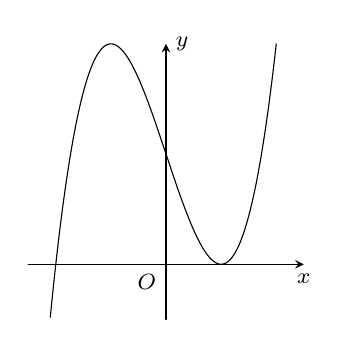
\begin{tikzpicture}[line cap=round, line join=round, font=\footnotesize, >=stealth, scale=0.7]
			\tikzset{label style/.style={font=\footnotesize}}
			\draw[->] (-2.5,0)--(2.5,0) node[below]{$x$};
			\draw[->] (0,-1)--(0,4) node[right]{$y$};
			\draw[smooth, samples=100] plot[domain=-2.1:2] (\x, {(\x)^3-3*(\x)+2});
			\node at (0,0)[below left]{$O$}; 
		\end{tikzpicture}
	}
	\loigiai{
		Đồ thị hình vẽ là đồ thị hàm số bậc ba có hệ số $a>0$ nên chỉ có hàm số $y=x^3-3x+2$ thỏa mãn điều kiện trên.}
\end{ex}

\begin{ex}%[2D1Y5-1]
	[Mã 102 - 2020 Lần 2]
	\immini{
		Đồ thị của hàm số nào dưới đây có dạng như đường cong trong hình bên?
		\choice
		{$ y=-x^4+2x^2-1$}
		{$ y=x^4-2x^2-1$}
		{$ y=x^3-3x^2-1$}
		{\True $ y=-x^3+3x^2-1$}
	}{
		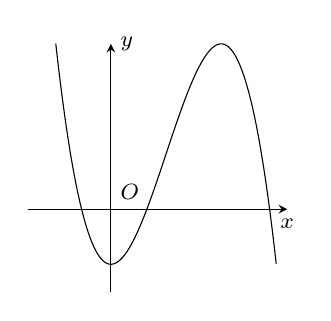
\begin{tikzpicture}[line cap=round, line join=round, font=\footnotesize, >=stealth, scale=0.7]
			\tikzset{label style/.style={font=\footnotesize}}
			\draw[->] (-1.5,0)--(3.2,0) node[below]{$x$};
			\draw[->] (0,-1.5)--(0,3) node[right]{$y$};
			\draw[smooth, samples=100] plot[domain=-1:3] (\x, {-(\x)^3+3*(\x)^2-1});
			\node at (0,0)[above right]{$O$}; 
		\end{tikzpicture}
	}	
	\loigiai{
		Dựa vào đồ thị có dạng đồ thị của hàm số bậc ba có hệ số $a<0$ nên đáp án $y=-x^3+3x^2-1$ đúng.}
\end{ex}

\begin{ex}%[2D1Y5-1]
	[Mã 103 - 2020 Lần 2]
	\immini{
		Đồ thị của hàm số dưới đây có dạng như đường cong bên?
		\choice
		{\True $y=x^3-3x+1$}
		{$y=x^4-2x^2+1$}
		{$y=-x^4+2x^2+1$}
		{$y=-x^3+3x+1$}
	}{
		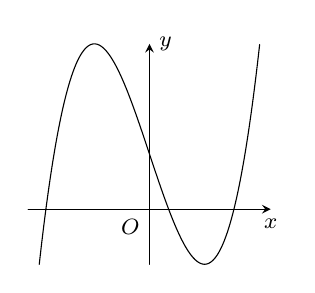
\begin{tikzpicture}[line cap=round, line join=round, font=\footnotesize, >=stealth, scale=0.7]
			\tikzset{label style/.style={font=\footnotesize}}
			\draw[->] (-2.2,0)--(2.2,0) node[below]{$x$};
			\draw[->] (0,-1)--(0,3) node[right]{$y$};
			\draw[smooth, samples=100] plot[domain=-2:2] (\x, {(\x)^3-3*(\x)+1});
			\node at (0,0)[below left]{$O$}; 
		\end{tikzpicture}
	}	
	\loigiai{
		Đồ thị đã cho là đồ thị hàm bậc ba, với hệ số $a>0$.
	}
\end{ex}

\begin{ex}%[2D1Y5-1]
	[Mã 104 - 2020 Lần 2]
	\immini{
		Đồ thị của hàm số nào dưới đây có dạng như đường cong trong hình bên?
		\choice
		{$ y=x^4+2x^2$}
		{$ y=-x^3-3x$}
		{\True $ y=x^3-3x$}
		{$ y=-x^4+2x^2$}
	}{
		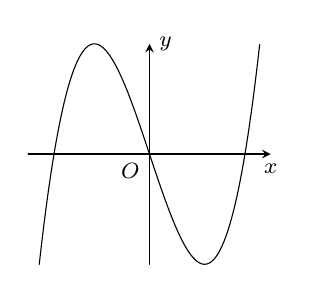
\begin{tikzpicture}[line cap=round, line join=round, font=\footnotesize, >=stealth, scale=0.7]
			\tikzset{label style/.style={font=\footnotesize}}
			\draw[->] (-2.2,0)--(2.2,0) node[below]{$x$};
			\draw[->] (0,-2)--(0,2) node[right]{$y$};
			\draw[smooth, samples=100] plot[domain=-2:2] (\x, {(\x)^3-3*(\x)});
			\node at (0,0)[below left]{$O$}; 
		\end{tikzpicture}
	}
	\loigiai{
		Đây là đồ thị của hàm số bậc ba với hệ số $ a>0$, đó là hàm số $ y=x^3-3x$.
	}
\end{ex}

\begin{ex}%[2D1Y5-1]
	[Mã 102 - 2018]
	\immini{
		Đường cong trong hình vẽ bên là đồ thị của hàm số nào dưới đây?
		\choice
		{$ y=-x^3+x^2-1$}
		{$ y=-x^4+2x^2-1$}
		{$ y=x^3-x^2-1$}
		{\True $ y=x^4-2x^2-1$}
	}{
		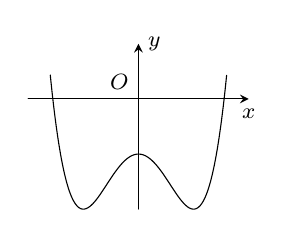
\begin{tikzpicture}[line cap=round, line join=round, font=\footnotesize, >=stealth, scale=0.7]
			\tikzset{label style/.style={font=\footnotesize}}
			\draw[->] (-2,0)--(2,0) node[below]{$x$};
			\draw[->] (0,-2)--(0,1) node[right]{$y$};
			\draw[smooth, samples=100] plot[domain=-1.6:1.6] (\x, {(\x)^4-2*(\x)^2-1});
			\node at (0,0)[above left]{$O$}; 
		\end{tikzpicture}
	}
	\loigiai{
		Dựa vào hình vẽ suy ra hàm số đã cho có $ 3$ cực trị$\to $ loại $y=x^3-x^2-1$.\\
		Mặt khác nhánh bên tay phải của đồ thị hàm số đi lên suy ra hệ số $a>0$, nên chọn $y=x^4-2x^2-1$.}
\end{ex}

\begin{ex}%[2D1Y5-1]
	[Đề Tham Khảo 2019]
	\immini{
		Đường con trong hình vẽ bên là đồ thị của hàm số nào dưới đây?
		\choice
		{$ y=\dfrac{2x-1}{x-1}$}
		{\True $ y=\dfrac{x+1}{x-1}$}
		{$ y=x^4+x^2+1$}
		{$ y=x^3-3x-1$}
	}{
		\begin{tikzpicture}[line cap=round, line join=round, font=\footnotesize, >=stealth, scale=0.7]
			\tikzset{label style/.style={font=\footnotesize}}
			\draw[->] (-3,0)--(5,0) node[below]{$x$};
			\draw[->] (0,-3)--(0,4.5) node[right]{$y$};
			\draw[smooth, samples=100] plot[domain=-3:0.5] (\x, {(\x+1)/(\x-1)});
			\draw[smooth, samples=100] plot[domain=1.6:5] (\x, {(\x+1)/(\x-1)});
			\draw (1,-3)--(1,4.5) (-3,1)--(5,1);
			\draw[fill=black] (0,0) circle (1pt) node[above left]{$O$}
			(1,0) circle (1pt) node[below right]{$1$}
			(0,1) circle (1pt) node[above left]{$1$}; 
		\end{tikzpicture}	
	}
	\loigiai{
		Từ đồ thị ta suy ra đồ thị của hàm phân thức có tiệm cận đứng và ngang lần lượt là các đường thẳng $x=1$; $y=1$.
	}
\end{ex}

\begin{ex}%[2D1Y5-1]
	[Mã 110 - 2017]
	\immini{
		Đường cong ở hình bên dưới là đồ thị của một trong bốn hàm số dưới đây. Hàm số đó là hàm số nào?
		\choice
		{$ y=-x^3+3x^2+1$}
		{\True $ y=x^3-3x^2+3$}
		{$ y=-x^4+2x^2+1$}
		{$ y=x^4-2x^2+1$}
	}{
		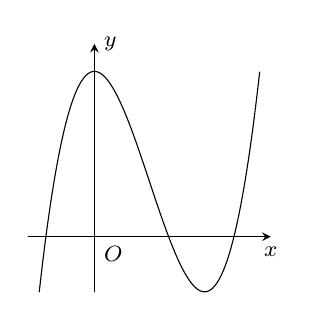
\begin{tikzpicture}[line cap=round, line join=round, font=\footnotesize, >=stealth, scale=0.7]
			\tikzset{label style/.style={font=\footnotesize}}
			\draw[->] (-1.2,0)--(3.2,0) node[below]{$x$};
			\draw[->] (0,-1)--(0,3.5) node[right]{$y$};
			\draw[smooth, samples=100] plot[domain=-1:3] (\x, {(\x)^3-3*(\x)^2+3});
			\node at (0,0)[below right]{$O$}; 
		\end{tikzpicture}
	}
	\loigiai{
		Dựa vào đồ thị ta thấy đây là hình ảnh đồ thị của hàm số bậc ba nên loại đáp án $y=-x^4+2x^2+1$ và $y=x^4-2x^2+1$.\\
		Mặt khác dựa vào đồ thị ta có $\lim\limits_{x\to+\infty}y=+\infty$ nên hệ số của $x^3$ dương nên ta chọn đáp án $ y=x^3-3x^2+3$.}
\end{ex}

\begin{ex}%[2D1Y5-1]
	[Mã 103 - 2019]
	\immini{
		Đồ thị hàm số nào dưới đây có dạng như đường cong trong hình vẽ bên?
		\choice
		{$y=x^3-3x^2-2$}
		{\True $y=x^4-2x^2-2$}
		{$y=-x^3+3x^2-2$}
		{$y=-x^4+2x^2-2$}
	}{
		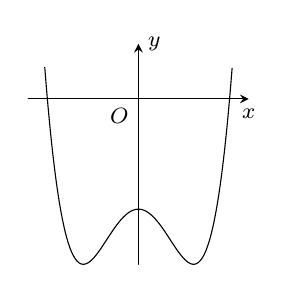
\begin{tikzpicture}[line cap=round, line join=round, font=\footnotesize, >=stealth, scale=0.7]
			\tikzset{label style/.style={font=\footnotesize}}
			\draw[->] (-2,0)--(2,0) node[below]{$x$};
			\draw[->] (0,-3)--(0,1) node[right]{$y$};
			\draw[smooth, samples=100] plot[domain=-1.7:1.7] (\x, {(\x)^4-2*(\x)^2-2});
			\node at (0,0)[below left]{$O$}; 
		\end{tikzpicture}
	}
	\loigiai{
		Quan sát đồ thị ta thấy đây là đồ thị của hàm số $y=a{x^4}+b{x^2}+c~\left(a>0\right)$.}
\end{ex}

\begin{ex}%[2D1Y5-1]
	[Đề Tham Khảo 2017]
	Cho đường cong hình vẽ dưới đây là đồ thị của một hàm số trong bốn hàm số được liệt kê ở bốn phương án A, B, C, D dưới đây. Hỏi đó là hàm số nào?
	\begin{center}
		\begin{tikzpicture}[line cap=round, line join=round, font=\footnotesize, >=stealth, scale=0.7]
			\tikzset{label style/.style={font=\footnotesize}}
			\draw[->] (-5,0)--(4,0) node[below]{$x$};
			\draw[->] (0,-3)--(0,6) node[right]{$y$};
			\draw[smooth, samples=100] plot[domain=-1.75:-5] (\x, {(2*\x-1)/(\x+1)});
			\draw[smooth, samples=100] plot[domain=-0.4:4] (\x, {(2*\x-1)/(\x+1)});
			\draw (-1,6)--(-1,-3) (-5,2)--(4,2);
			\draw[fill=black] (0,0) circle (1pt) node[above left]{$O$}
			(-1,0) circle (1pt) node[below left]{$-1$}
			(0,2) circle (1pt) node[above right]{$2$}
			(0,-1) circle (1pt) node[right]{$-1$};
		\end{tikzpicture}
	\end{center}
	\choice
	{$ y=\dfrac{2x+1}{x-1}$}
	{$ y=\dfrac{2x+3}{x+1}$}
	{\True $ y=\dfrac{2x-1}{x+1}$}
	{$ y=\dfrac{2x-2}{x-1}$}
	\loigiai{
		Dựa vào đồ thị suy ra tiệm cận đứng $ x=-1$ loại $ y=\dfrac{2x+1}{x-1}$ và $ y=\dfrac{2x-2}{x-1}$.\\
		Đồ thị hàm số giao với trục hoành có hoành độ dương suy ra chọn $ y=\dfrac{2x-1}{x+1}$.
	}
\end{ex}

\begin{ex}%[2D1Y5-1]
	[Đề Minh Họa 2017]
	\immini{
		Đường cong trong hình bên là đồ thị của một hàm số trong bốn hàm số
		được liệt kê ở bốn phương án A, B, C, D dưới đây. Hỏi hàm số đó là hàm số nào?
		\choice
		{\True $ y=x^3-3x+1$}
		{$ y=-x^3+3x+1$}
		{$ y=x^4-x^2+1$}
		{$ y=-x^2+x-1$}
	}{
		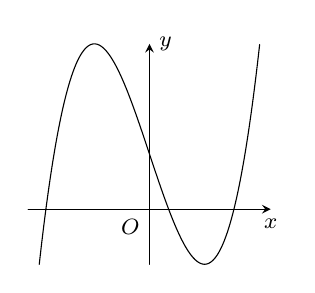
\begin{tikzpicture}[line cap=round, line join=round, font=\footnotesize, >=stealth, scale=0.7]
			\tikzset{label style/.style={font=\footnotesize}}
			\draw[->] (-2.2,0)--(2.2,0) node[below]{$x$};
			\draw[->] (0,-1)--(0,3) node[right]{$y$};
			\draw[smooth, samples=100] plot[domain=-2:2] (\x, {(\x)^3-3*(\x)+1});
			\node at (0,0)[below left]{$O$}; 
		\end{tikzpicture}
	}
	\loigiai{
		Từ đồ thị $\lim\limits_{x\to+\infty}y=+\infty$ và đây là đồ thị hàm bậc ba nên ta chọn phương án $ y=x^3-3x+1$.}
\end{ex}

\begin{ex}%[2D1Y5-1]
	[Mã 101 - 2019]
	\immini{
		Đồ thị của hàm số nào dưới đây có dạng như đường cong trong hình vẽ bên?
		\choice
		{\True $ y=x^3-3x^2+3$}
		{$ y=-x^3+3x^2+3$}
		{$ y=x^4-2x^2+3$}
		{$ y=-x^4+2x^2+3$}
	}{
		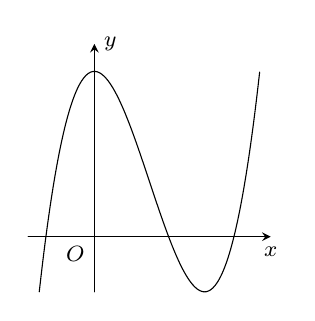
\begin{tikzpicture}[line cap=round, line join=round, font=\footnotesize, >=stealth, scale=0.7]
			\tikzset{label style/.style={font=\footnotesize}}
			\draw[->] (-1.2,0)--(3.2,0) node[below]{$x$};
			\draw[->] (0,-1)--(0,3.5) node[right]{$y$};
			\draw[smooth, samples=100] plot[domain=-1:3] (\x, {(\x)^3-3*(\x)^2+3});
			\node at (0,0)[below left]{$O$}; 
		\end{tikzpicture}
	}
	\loigiai{
		Dạng hàm bậc ba nên loại $ y=x^4-2x^2+3$ và $ y=-x^4+2x^2+3$.\\
		Từ đồ thị ta có $ a>0$. Do đó loại $y=-x^3+3x^2+3$.}
\end{ex}

\begin{ex}%[2D1Y5-1]
	[Mã 101 - 2018]
	\immini{
		Đường cong trong hình vẽ bên là đồ thị của hàm số nào dưới đây?
		\choice
		{$ y=x^3-3x^2-1$}
		{$ y=-x^3+3x^2-1$}
		{\True $ y=-x^4+3x^2-1$}
		{$ y=x^4-3x^2-1$}
	}{
		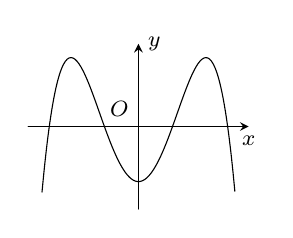
\begin{tikzpicture}[line cap=round, line join=round, font=\footnotesize, >=stealth, scale=0.7]
			\tikzset{label style/.style={font=\footnotesize}}
			\draw[->] (-2,0)--(2,0) node[below]{$x$};
			\draw[->] (0,-1.5)--(0,1.5) node[right]{$y$};
			\draw[smooth, samples=100] plot[domain=-1.75:1.75] (\x, {-(\x)^4+3*(\x)^2-1});
			\node at (0,0)[above left]{$O$}; 
		\end{tikzpicture}
	}
	\loigiai{
		Nhìn đồ thị khẳng định đồ thị hàm trùng phương loại $y=x^3-3x^2-1$ và $y=-x^3+3x^2-1$.\\
		$\lim\limits_{x\to\pm\infty}y=-\infty$ nên chọn $y=-x^4+3x^2-1$.}
\end{ex}

\begin{ex}%[2D1Y5-1]
	[Mã 104 - 2019]
	\immini{
		Đồ thị hàm số nào dưới đây có dạng như đường cong trong hình vẽ bên?
		\choice
		{$ y=2x^4-4x^2+1$}
		{$ y=-2x^3+3x+1$}
		{$ y=2x^3-3x+1$}
		{\True $ y=-2x^4+4x^2+1$}
	}{
		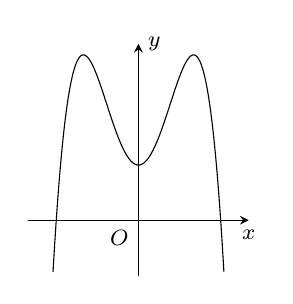
\begin{tikzpicture}[line cap=round, line join=round, font=\footnotesize, >=stealth, scale=0.7]
			\tikzset{label style/.style={font=\footnotesize}}
			\draw[->] (-2,0)--(2,0) node[below]{$x$};
			\draw[->] (0,-1)--(0,3.2) node[right]{$y$};
			\draw[smooth, samples=100] plot[domain=-1.55:1.55] (\x, {-2*(\x)^4+4*(\x)^2+1});
			\node at (0,0)[below left]{$O$}; 
		\end{tikzpicture}
	}
	\loigiai{
		Dạng đồ thị hình bên là đồ thị hàm số trùng phương $ y=a{x^4}+b{x^2}+c$ có hệ số $ a<0$.\\
		Do đó, chỉ có đồ thị ở đáp án $y=-2x^4+4x^2+1$ là thỏa mãn.}
\end{ex}
\begin{ex}%[2D1Y5-1]
	[Mã 102 2019] 
	\immini{
		Đồ thị của hàm số nào dưới đây có dạng như đường cong trong hình vẽ bên
	\choice
	{\True $y=-x^3+3x+1$}
	{$y=x^3-3x+1$}
	{$y=x^4-2x^2+1$}
	{$y=-x^4+2x^2+1$}
	}{
		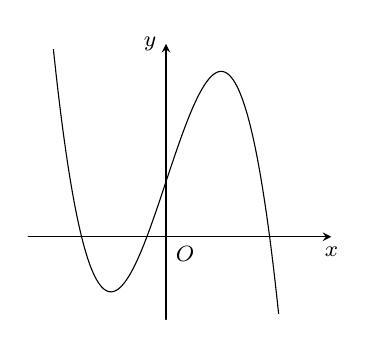
\begin{tikzpicture}[scale=0.7, font=\footnotesize, line join=round, line cap=round,>=stealth]
			\def\a{-1} \def\b{0} \def\c{3} \def\d{1} % Hệ số
			\def\xmin{-2.5} \def\xmax{3}
			\def\ymin{-1.5} \def\ymax{3.5} 
			\draw[->] (\xmin,0)--(\xmax,0) node [below]{$x$};
			\draw[->] (0,\ymin)--(0,\ymax) node [left]{$y$};
			\node at (0,0) [below right]{$O$};
			\clip (\xmin+0.1,\ymin+0.1) rectangle (\xmax-0.1,\ymax-0.1);
			\draw[smooth,samples=300] plot(\x,{\a*(\x)^3+\b*(\x)^2+\c*(\x)+\d});
		\end{tikzpicture}
	}
	\loigiai{
		Trong bốn hàm số đã cho thì chỉ có hàm số $y=-x^3+3x+1$ (hàm số đa thức bậc ba với hệ số $a<0$) có dạng đồ thị như đường cong trong hình.}
\end{ex}
\begin{ex}%[2D1Y5-1]
	[Mã 104 2018]
	\immini{
		Đường cong trong hình vẽ bên là đồ thị của hàm số nào dưới đây?
	\choice
	{$y=x^4-x^2-2$}
	{$y=-x^4+x^2-2$}
	{\True $y=-x^3+3x^2-2$}
	{$y=x^3-3x^2-2$}
	}{
		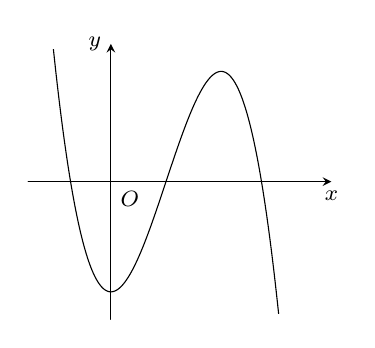
\begin{tikzpicture}[scale=0.7, font=\footnotesize, line join=round, line cap=round,>=stealth]
			\def\a{-1} \def\b{3} \def\c{0} \def\d{-2} % Hệ số
			\def\xmin{-1.5} \def\xmax{4}
			\def\ymin{-2.5} \def\ymax{2.5} 
			\draw[->] (\xmin,0)--(\xmax,0) node [below]{$x$};
			\draw[->] (0,\ymin)--(0,\ymax) node [left]{$y$};
			\node at (0,0) [below right]{$O$};
			\clip (\xmin+0.1,\ymin+0.1) rectangle (\xmax-0.1,\ymax-0.1);
			\draw[smooth,samples=300] plot(\x,{\a*(\x)^3+\b*(\x)^2+\c*(\x)+\d});
		\end{tikzpicture}
	}
	\loigiai{
		Dựa trên hình dáng đồ thị, ta loại $y=x^3-3x^2-2$ và $y=x^4-x^2-2$.\\
		Mặt khác từ đồ thị, ta thấy $\lim\limits_{x\to+\infty} y=-\infty$ nên loại $y=-x^4+x^2-2$.}
\end{ex}
\begin{ex}%[2D1B5-1]%Câu 23.
	[Mã 103 2018]\immini{ Đường cong trong hình vẽ là đồ thị của hàm số nào dưới đây?		
		\choice
		{\True $y=x^3-3x-1$}
		{$y=x^4-3x^2-1$}
		{$y=-x^3-3x-1$}
		{$y=-x^4+x^2-1$}}{		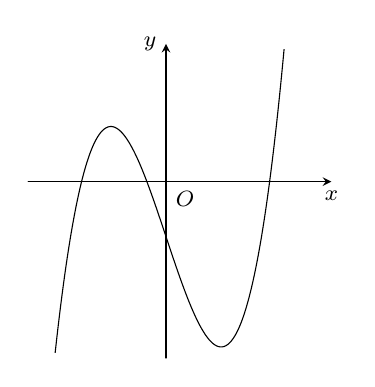
\begin{tikzpicture}[scale=0.7, font=\footnotesize, line join=round, line cap=round,>=stealth]
			\def\a{1} \def\b{0} \def\c{-3} \def\d{-1} % Hệ số
			\def\xmin{-2.5} \def\xmax{3}
			\def\ymin{-3.2} \def\ymax{2.5} 
			\draw[->] (\xmin,0)--(\xmax,0) node [below]{$x$};
			\draw[->] (0,\ymin)--(0,\ymax) node [left]{$y$};
			\node at (0,0) [below right]{$O$};
			\clip (\xmin+0.1,\ymin+0.1) rectangle (\xmax-0.1,\ymax-0.1);
			\draw[smooth,samples=300] plot(\x,{\a*(\x)^3+\b*(\x)^2+\c*(\x)+\d});
	\end{tikzpicture}}
	\loigiai{
		Dựa trên hình dáng đồ thị, ta loại các hàm số $y=x^4-3x^2-1$ và $y=-x^4+x^2-1$.\\
		Mặt khác từ đồ thị, ta thấy $\lim\limits_{x\to-\infty} y=-\infty$ nên loại $y=-x^3-3x-1$.}
\end{ex}
\begin{ex}%[2D1B5-1]%Câu 24.
	[Mã 123 2017]
	\immini{
		Đường cong ở hình bên là đồ thị của một trong bốn hàm số dưới đây. Hàm số đó là hàm số nào?
		\choice
		{\True $y=x^4-x^2-1$}
		{$y=-x^4+x^2-1$}
		{$y=x^3-x^2-1$}
		{$y=-x^3+x^2-1$}}{	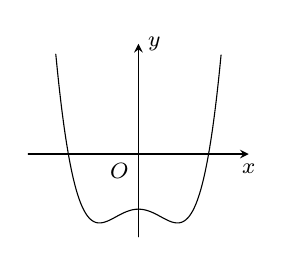
\begin{tikzpicture}[line cap=round, line join=round, font=\footnotesize, >=stealth, scale=0.7]
			\tikzset{label style/.style={font=\footnotesize}}
			\draw[->] (-2,0)--(2,0) node[below]{$x$};
			\draw[->] (0,-1.5)--(0,2) node[right]{$y$};
			\draw[smooth, samples=100] plot[domain=-1.5:1.5] (\x, {(\x)^4-1*(\x)^2-1});
			\node at (0,0)[below left]{$O$}; 
	\end{tikzpicture}}
	\loigiai{
		Đây là hình dáng của đồ thị hàm bậc bốn trùng phương có hệ số $a>0$ nên ta loại các hàm số 	$y=-x^4+x^2-1$, $y=x^3-x^2-1$, 	$y=-x^3+x^2-1$.}
\end{ex}
\begin{ex}%[2D1B5-1]%Câu 25.
	[Đề Tham Khảo 2018]
	\immini{
		Đường cong trong hình bên là của đồ thị hàm số nào dưới đây?
		\choice
		{$y=x^3-3x^2+2$}
		{$y=-x^3+3x^2+2$}
		{\True $y=-x^4+2x^2+2$}
		{$y=x^4-2x^2+2$}}{	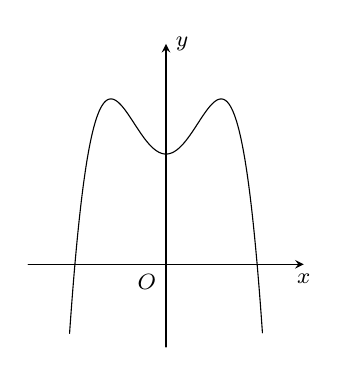
\begin{tikzpicture}[line cap=round, line join=round, font=\footnotesize, >=stealth, scale=0.7]
			\tikzset{label style/.style={font=\footnotesize}}
			\draw[->] (-2.5,0)--(2.5,0) node[below]{$x$};
			\draw[->] (0,-1.5)--(0,4) node[right]{$y$};
			\draw[smooth, samples=300] plot[domain=-1.75:1.75] (\x, {-1*(\x)^4+2*(\x)^2+2});
			\node at (0,0)[below left]{$O$}; 
	\end{tikzpicture}}
	\loigiai{
		Đồ thị hàm số trên là đồ thị hàm số trùng phương có $3$ cực trị và có $a<0$ nên loại các hàm số $y=x^3-3x^2+2$,
		$y=-x^3+3x^2+2$, 
		$y=x^4-2x^2+2$.}
\end{ex}
\begin{ex}%[2D1B5-1]%Câu 26.
	[Mã 123 2017]
	\immini{ Đường cong ở hình bên là đồ thị của hàm số $y=\dfrac{ax+b}{cx+d}$ với $a,b,c,d$ là các số thực. Mệnh đề nào dưới đây đúng?
		\choice
		{$y'<0,\forall x\in\mathbb{R}$}
		{$y'>0,\forall x\neq 1$}
		{\True$y'<0,\forall x\neq 1$}
		{$y'>0,\forall x\in\mathbb{R}$}}{	\begin{tikzpicture}[line cap=round, line join=round, font=\footnotesize, >=stealth, scale=0.6]
			\tikzset{label style/.style={font=\footnotesize}}
			\draw[->] (-4,0)--(5,0) node[below]{$x$};
			\draw[->] (0,-5)--(0,7) node[right]{$y$};
			\draw[smooth, samples=100] plot[domain=-4:0.65] (\x, {(\x+1)/(\x-1)});
			\draw[smooth, samples=100] plot[domain=1.35:5] (\x, {(\x+1)/(\x-1)});
			\draw (1,7)--(1,-5) (-4,1)--(5,1);
			\draw[fill=black] (0,0) circle (1pt) node[above left]{$O$}
			(-1,0) circle (1pt) node[below left]{$-1$}
			(0,1) circle (1pt) node[above right]{$1$}
			(0,-1) circle (1pt) node[right]{$-1$};
	\end{tikzpicture}}
	\loigiai{
		Đồ thị đã cho nhận đường thẳng $x=1$ làm tiệm cận đứng nên hàm số ta có \\
		Điều kiện xác định của hàm số là $x\neq 1$.\\
		Đây là đồ thị của hàm nghịch biến.\\
		Từ đó ta được $y'<0,\forall x\neq 1$.}
\end{ex}
\begin{ex}%[2D1B5-1]%Câu 27.
	[Mã 105 2017]
	\immini{Đường cong ở hình bên là đồ thị của hàm số $y=\dfrac{ax+b}{cx+d}$ với $a,b,c,d$ là các số thực. Mệnh đề nào dưới đây đúng?
		\choice
		{$y'>0,\forall x\neq 1$}
		{$y'<0,\forall x\neq 1$}
		{\True $y'<0,\forall x\neq 2$}
		{$y'>0,\forall\neq 2$}}{\begin{tikzpicture}[line cap=round, line join=round, font=\footnotesize, >=stealth, scale=0.6]
			\tikzset{label style/.style={font=\footnotesize}}
			\draw[->] (-4,0)--(7,0) node[below]{$x$};
			\draw[->] (0,-5)--(0,7) node[right]{$y$};
			\draw[smooth, samples=100] plot[domain=-4:1.5] (\x, {(\x+1)/(\x-2)});
			\draw[smooth, samples=100] plot[domain=2.5:7] (\x, {(\x+1)/(\x-2)});
			\draw (2,7)--(2,-5) (-4,1)--(7,1);
			\draw[fill=black] (0,0) circle (1pt) node[above left]{$O$}
			(2,0) circle (1pt) node[above right]{$2$}
			(0,1) circle (1pt) node[above right]{$1$};
	\end{tikzpicture}}
	\loigiai{
		Đồ thị đã cho nhận đường thẳng $x=2$ làm tiệm cận đứng và là đồ thị của hàm số nghịch biến trên mỗi khoảng $(-\infty;2),\,(2;+\infty)$ nên $y'<0,\forall x\neq 2$.}
\end{ex}
\begin{ex}%[2D1B5-1]%Câu 28.
	[THPT Yên Phong 1 Bắc Ninh 2019]
	\immini{Hình vẽ sau đây là đồ thị của một trong bốn hàm số cho ở các đáp án $A$, $B$, $C$, $D$. Hỏi đó là hàm số nào?
		\choice
		{$y=x^3+2x+1$}
		{$y=x^3-2x^2+1$}
		{\True $y=x^3-2x+1$}
		{$y=-x^3+2x+1$}}{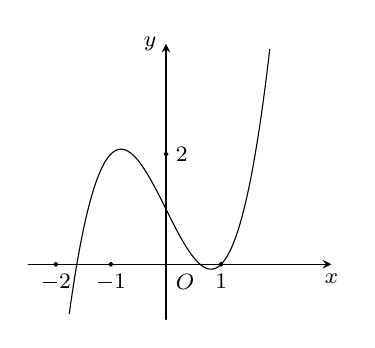
\begin{tikzpicture}[scale=0.7, font=\footnotesize, line join=round, line cap=round,>=stealth]
			\def\a{1} \def\b{0} \def\c{-2} \def\d{1} % Hệ số
			\def\xmin{-2.5} \def\xmax{3}
			\def\ymin{-1.0} \def\ymax{4} 
			\draw[->] (\xmin,0)--(\xmax,0) node [below]{$x$};
			\draw[->] (0,\ymin)--(0,\ymax) node [left]{$y$};
			\node at (0,0) [below right]{$O$};
			\clip (\xmin+0.1,\ymin+0.1) rectangle (\xmax-0.1,\ymax-0.1);
			\draw[smooth,samples=300] plot(\x,{\a*(\x)^3+\b*(\x)^2+\c*(\x)+\d});
			\draw[fill=black](-2,0) circle (1pt) node[below]{$-2$}
			(0,2) circle (1pt) node[right]{$2$}
			(1,0) circle (1pt) node[below]{$1$}
			(-1,0) circle (1pt) node[below]{$-1$};
	\end{tikzpicture}}
	\loigiai{
		Dựa vào đồ thị, ta có $\lim\limits_{x\to+\infty} y=+\infty$, loại hàm số  $y=-x^3+2x+1$.\\
		Xét hàm số $y=x^3+2x+1$, ta có $y'=3x^2+2>0,\forall x\in\mathbb{R}$, hàm số không có cực tri.\\
		Xét hàm số $y=x^3-2x^2+1$ có $y'=3x^2-6x$ và $y'$ đổi dấu khi đi qua các điểm $x=0, x=2$ nên hàm số đạt cực tri tại $x=0$ và $x=2$.\\
		Vậy phương án đúng là $C$.}
\end{ex}
\begin{ex}%[2D1B5-1]%Câu 29.
	[Sở Cần Thơ - 2019]
	\immini{Hình vẽ bên là đồ thị của hàm số nào trong các hàm số sau?
		\choice
		{$y=\dfrac{x-1}{x+1}$}
		{\True $y=\dfrac{2x+1}{x+1}$}
		{$y=\dfrac{2x-3}{x+1}$}
		{$y=\dfrac{2x+5}{x+1}$}}{\begin{tikzpicture}[line cap=round, line join=round, font=\footnotesize, >=stealth, scale=0.6]
			\tikzset{label style/.style={font=\footnotesize}}
			\draw[->] (-6,0)--(5,0) node[below]{$x$};
			\draw[->] (0,-3)--(0,7) node[right]{$y$};
			\draw[smooth, samples=100] plot[domain=-6:-1.2] (\x, {(2*\x+1)/(\x+1)});
			\draw[smooth, samples=100] plot[domain=-0.8:5] (\x, {(2*\x+1)/(\x+1)});
			\draw (-1,7)--(-1,-3) (-6,2)--(5,2);
			\draw[fill=black] (0,0) circle (1pt) node[below right]{$O$}
			(0,1) circle (1pt) node[right]{$1$}
			(-1,0) circle (1pt) node[below left]{$-1$}
			(0,2) circle (1pt) node[above right]{$2$};
	\end{tikzpicture}}
	\loigiai{
		Đồ thị hàm số cắt trục $Oy$ tai điểm có tọa độ $(0; 1)$. Ta thấy hàm số $y=\dfrac{2x+1}{x+1}$ có đồ thị thỏa mãn hình đã cho.
	}
\end{ex}
\begin{ex}%[2D1B5-1]%Câu 30.
	[SGD Nam Định]
	\immini{ Đường cong trong hình là đồ thị của hàm số nào dưới đây?
		\choice
		{\True $y=\dfrac{x-1}{x+1}$}
		{$y=\dfrac{-2x+1}{2x+2}$}
		{$y=x^4-3x^2$}
		{$y=x^3-3x^2$}}{\begin{tikzpicture}[line join=round, line cap=round,>=stealth,scale=0.8]
			\tikzset{every node/.style={scale=0.9}}
			\draw[->] (-5,0)--(3.1,0) node[below left] {$x$};
			\draw[->] (0,-3.1)--(0,5) node[below left] {$y$};
			\draw (0,0) node [below left] {$O$};
			\foreach \x in {-1}
			\draw[thin] (\x,1pt)--(\x,-1pt) node [below left] {$\x$};
			\foreach \y in {1}
			\draw[thin] (1pt,\y)--(-1pt,\y) node [above left] {$\y$};
			\draw (-0.99,-3)--(-0.99,5);
			\begin{scope}
				\clip (-5,-3) rectangle (3,5);
				\draw[samples=200,domain=-5:-1.01,smooth,variable=\x] plot (\x,{(1*(\x)+-1)/(1*(\x)+1)});
				\draw[samples=200,domain=-0.99:3,smooth,variable=\x] plot (\x,{(1*(\x)+-1)/(1*(\x)+1)});
				\draw[samples=200,domain=-5:-1.01,smooth,variable=\x] plot (\x,{(1*(\x)-1)/(1*(\x)+1)});
				\draw[samples=200,domain=-0.99:3,smooth,variable=\x] plot (\x,{(1*(\x)-1)/(1*(\x)+1)});
				\draw(-5,1/1)--(3,1/1);
			\end{scope}
	\end{tikzpicture}}
	\loigiai{
		Hình vẽ trên là đồ thị của hàm số dạng $y=\dfrac{ax+b}{cx+d}\left(c\neq 0; ad-bc\neq 0\right)$ nên loại các hàm số $y=x^4-3x^2$,
		$y=x^3-3x^2$.\\
		Ta thấy: Đồ thị có đường tiệm cận đứng là $x=-1$ và đường tiệm cận ngang là $y=1$ nên loại hàm số $y=\dfrac{-2x+1}{2x+2}$.}
\end{ex}
\begin{ex}%[2D1B5-1]%Câu 31.
	[Sở Gia Lai 2019]
	\immini{Đường cong trong hình vẽ bên là đồ thị của hàm số nào sau đây?
		\choice
		{$y=-x^3+3x+1$}
		{$y=x^4-x^2+1$}
		{$y=-x^2+x-1$}
		{\True $y=x^3-3x+1$}
	}{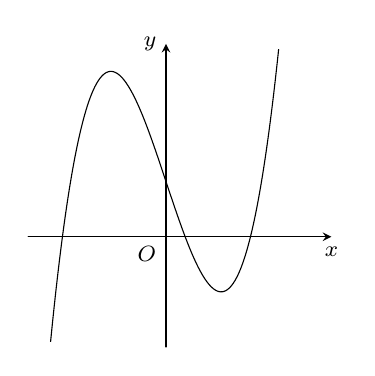
\begin{tikzpicture}[scale=0.7, font=\footnotesize, line join=round, line cap=round,>=stealth]
			\def\a{1} \def\b{0} \def\c{-3} \def\d{1} % Hệ số
			\def\xmin{-2.5} \def\xmax{3}
			\def\ymin{-2.0} \def\ymax{3.5} 
			\draw[->] (\xmin,0)--(\xmax,0) node [below]{$x$};
			\draw[->] (0,\ymin)--(0,\ymax) node [left]{$y$};
			\node at (0,0) [below left]{$O$};
			\clip (\xmin+0.1,\ymin+0.1) rectangle (\xmax-0.1,\ymax-0.1);
			\draw[smooth,samples=300] plot(\x,{\a*(\x)^3+\b*(\x)^2+\c*(\x)+\d});
	\end{tikzpicture}}
	\loigiai{
		Đồ thị đã cho có hình dạng của đồ thị hàm số bậc ba $y=ax^3+bx^2+cx+d$ nên loại các hàm số $y=x^4-x^2+1$, $y=-x^2+x-1$.\\
		Dựa vào đồ thị, ta có $\lim\limits_{x\to+\infty} y=+\infty\Rightarrow a>0$ nên loại hàm số $y=-x^3+3x+1$.}
\end{ex}
\begin{ex}%[2D1B5-1]%Câu 32.
	[Đề Minh Họa 2021]
	\immini{Đồ thị của hàm số nào dưới đây có dạng như đường cong trong hình sau
		\choice
		{$y=-x^4+2x^2-1$}
		{\True $y=x^4-2x^2-1$}
		{$y=x^3-3x^2-1$}
		{$y=-x^3+3x^2-1$}
	}{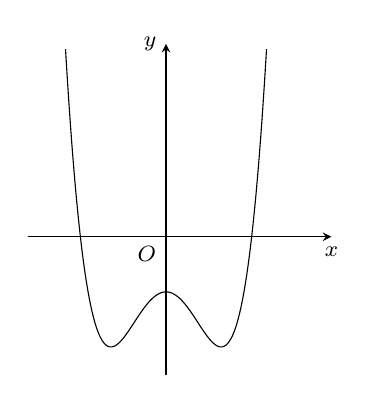
\begin{tikzpicture}[scale=0.7, font=\footnotesize, line join=round, line cap=round,>=stealth]
			\def\a{1} \def\b{-2} \def\c{0} \def\d{-1} % Hệ số
			\def\xmin{-2.5} \def\xmax{3}
			\def\ymin{-2.5} \def\ymax{3.5} 
			\draw[->] (\xmin,0)--(\xmax,0) node [below]{$x$};
			\draw[->] (0,\ymin)--(0,\ymax) node [left]{$y$};
			\node at (0,0) [below left]{$O$};
			\clip (\xmin+0.1,\ymin+0.1) rectangle (\xmax-0.1,\ymax-0.1);
			\draw[smooth,samples=300] plot(\x,{\a*(\x)^4+\b*(\x)^2+\c*(\x)+\d});
	\end{tikzpicture}}
	\loigiai{
		Dựa vào đồ thị hàm số ta thấy đây là đồ thị của hàm số bậc $4$ trùng phương với hệ số $a>0$. Do đó nhận đáp án $y=x^4-2x^2-1$.}
\end{ex}
\begin{ex}%[2D1B5-1]%Câu 33.
	[Mã 101 - 2021 Lần 1]
	\immini{
		Đồ thị của hàm số nào dưới đây có dạng như đường cong trong hình bên dưới?
		\choice
		{$y=-2x^4+4x^2-1$}
		{$y=-x^3+3x-1$}
		{\True$y=2x^4-4x^2-1$}
		{$y=x^3-3x-1$}
	}{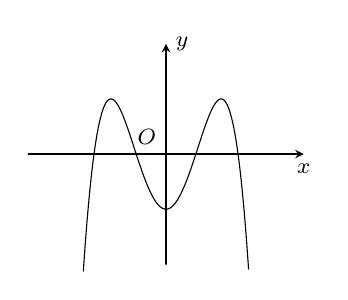
\begin{tikzpicture}[line cap=round, line join=round, font=\footnotesize, >=stealth, scale=0.7]
			\tikzset{label style/.style={font=\footnotesize}}
			\draw[->] (-2.5,0)--(2.5,0) node[below]{$x$};
			\draw[->] (0,-2)--(0,2) node[right]{$y$};
			\draw[smooth, samples=300] plot[domain=-1.5:1.5] (\x, {-2*(\x)^4+4*(\x)^2-1});
			\node at (0,0)[above left]{$O$}; 
	\end{tikzpicture}}
	\loigiai{
		Dựa vào dáng đồ thị, đây là hàm trùng phương nên loại các hàm số $y=-x^3+3x-1$,	$y=x^3-3x-1$.\\
		Dựa vào đồ thị, ta có $\lim\limits_{x\to+\infty} y=-\infty\Rightarrow a<0$ nên loại hàm số $y=2x^4-4x^2-1$.}
\end{ex}
\begin{ex}%[2D1B5-1]%Câu 34.
	[Mã 103 - 2021 - Lần 1]
	\immini{Đồ thị hàm số nào dưới đây có dạng như đường cong trong hình vẽ?
		\choice
		{$y=-x^3-2x+\dfrac{1}{2}$}
		{\True $y=x^3-2x+\dfrac{1}{2}$}
		{$y=-x^4+2x^2+\dfrac{1}{2}$}
		{$y=x^4+2x^2+\dfrac{1}{2}$}
	}{\begin{tikzpicture}[scale=0.7, font=\footnotesize, line join=round, line cap=round,>=stealth]
			\def\a{1} \def\b{0} \def\c{-2} \def\d{0.5} % Hệ số
			\def\xmin{-2.5} \def\xmax{3}
			\def\ymin{-2.0} \def\ymax{3.5} 
			\draw[->] (\xmin,0)--(\xmax,0) node [below]{$x$};
			\draw[->] (0,\ymin)--(0,\ymax) node [left]{$y$};
			\node at (0,0) [below left]{$O$};
			\clip (\xmin+0.1,\ymin+0.1) rectangle (\xmax-0.1,\ymax-0.1);
			\draw[smooth,samples=300] plot(\x,{\a*(\x)^3+\b*(\x)^2+\c*(\x)+\d});
	\end{tikzpicture}}
	\loigiai{
		Đồ thị đã cho là đồ thị hàm số bậc ba có hệ số bậc ba $a>0$. Đó là đồ thị của hàm số $y=x^3-2x+\dfrac{1}{2}$.}
\end{ex}
\begin{ex}%[2D1B5-1]%Câu 35.
	[Mã 102 - 2021 Lần 1]
	\immini{
		Đồ thị của hàm số nào dưới đây có dạng như đường cong trong hình vẽ?
		\choice
		{$y=x^3-3x+1$}
		{$y=-2x^4+4x^2+1$}
		{$y=-x^3+3x+1$}
		{\True $y=2x^4-4x^2+1$}
	}{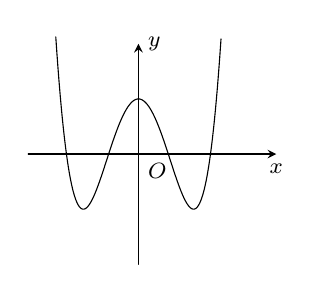
\begin{tikzpicture}[line cap=round, line join=round, font=\footnotesize, >=stealth, scale=0.7]
			\tikzset{label style/.style={font=\footnotesize}}
			\draw[->] (-2.0,0)--(2.5,0) node[below]{$x$};
			\draw[->] (0,-2)--(0,2) node[right]{$y$};
			\draw[smooth, samples=300] plot[domain=-1.5:1.5] (\x, {2*(\x)^4-4*(\x)^2+1});
			\node at (0,0)[below right]{$O$}; 
	\end{tikzpicture}}
	\loigiai{
		Đây là đồ thị hàm số bậc $4$ với hệ số $a>0$. Đó là đồ thị hàm số $y=2x^4-4x^2+1$.}
\end{ex}
\begin{ex}%[2D1B5-1]%Câu 36.
	[Mã 104 - 2021 Lần 1]
	\immini{ Đồ thị hàm số nào dưới đây có dạng như đường cong trong hình vẽ?
		\choice
		{$y=x^3-3x+1$}
		{$y=x^4+4x^2+1$}
		{\True $y=-x^3+3x+1$}
		{$y=-x^4+2x^2+1$}}{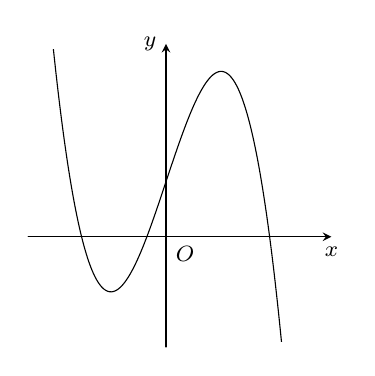
\begin{tikzpicture}[scale=0.7, font=\footnotesize, line join=round, line cap=round,>=stealth]
			\def\a{-1} \def\b{0} \def\c{3} \def\d{1} % Hệ số
			\def\xmin{-2.5} \def\xmax{3}
			\def\ymin{-2.0} \def\ymax{3.5} 
			\draw[->] (\xmin,0)--(\xmax,0) node [below]{$x$};
			\draw[->] (0,\ymin)--(0,\ymax) node [left]{$y$};
			\node at (0,0) [below right]{$O$};
			\clip (\xmin+0.1,\ymin+0.1) rectangle (\xmax-0.1,\ymax-0.1);
			\draw[smooth,samples=300] plot(\x,{\a*(\x)^3+\b*(\x)^2+\c*(\x)+\d});
	\end{tikzpicture}}
	\loigiai{
		Dựa vào đồ thị ta thấy đây là hàm số bậc $3$ có hệ số $a<0$, đó là đồ thị hàm số $y=-x^3+3x+1$.}
\end{ex}
\begin{ex}%[2D1B5-1]%Câu 37.
	[Mã 101 - 2021 Lần 1]
	\immini{Biết hàm số $y=\dfrac{x+a}{x+1}$ ($a$ là số thực cho trước, $a\neq 1$ có đồ thị như hình bên). Mệnh đề nào dưới đây đúng?
		\choice
		{$y'<0,\forall x\neq-1$}
		{\True $y'>0,\forall x\neq-1$}
		{$y'<0,\forall x\in\mathbb{R}$}
		{$y'>0,\forall x\in\mathbb{R}$}}{\begin{tikzpicture}[line cap=round, line join=round, font=\footnotesize, >=stealth, scale=0.6]
			\tikzset{label style/.style={font=\footnotesize}}
			\draw[->] (-6,0)--(5,0) node[below]{$x$};
			\draw[->] (0,-3)--(0,7) node[right]{$y$};
			\draw[smooth, samples=100] plot[domain=-6:-1.2] (\x, {(2*\x+1)/(\x+1)});
			\draw[smooth, samples=100] plot[domain=-0.8:5] (\x, {(2*\x+1)/(\x+1)});
			\draw (-1,7)--(-1,-3) (-6,2)--(5,2);
			\draw[fill=black] (0,0) circle (1pt) node[below right]{$O$}
			;
	\end{tikzpicture}}
	\loigiai{
		Ta có $y=\dfrac{x+a}{x+1} \Rightarrow y'=\dfrac{1-a}{(x+1)^2}>0,\forall x\neq-1 $.\\
		Từ đồ thị ta thấy hàm số đã ch đồng biến trên mỗi khoảng $(-\infty;-1)$, $(1;+\infty)$. \\
		Vậy khẳng định đúng là $y'>0,\forall x\neq-1$.}
\end{ex}
\begin{ex}%[2D1B5-1]%Câu 38.
	[Mã 103 - 2021 - Lần 1]
	\immini{ Biết hàm số $y=\dfrac{x+a}{x-1}$ ($a$ là số thực cho trước, $a\neq-1$) có đồ thị như trong hình vẽ.
		Mệnh đề nào dưới đây đúng?
		\choice
		{\True $y'>0,\forall x\neq 1$}
		{$y'>0,\forall x\in\mathbb{R}$}
		{$y'<0,\forall x\in\mathbb{R}$}
		{$y'<0,\forall x\neq 1$}}{\begin{tikzpicture}[line cap=round, line join=round, font=\footnotesize, >=stealth, scale=0.6]
			\tikzset{label style/.style={font=\footnotesize}}
			\draw[->] (-6,0)--(5,0) node[below]{$x$};
			\draw[->] (0,-3)--(0,7) node[right]{$y$};
			\draw[smooth, samples=100] plot[domain=-6:-1.2] (\x, {(2*\x+1)/(\x+1)});
			\draw[smooth, samples=100] plot[domain=-0.8:5] (\x, {(2*\x+1)/(\x+1)});
			\draw (-1,7)--(-1,-3) (-6,2)--(5,2);
			\draw[fill=black] (0,0) circle (1pt) node[below right]{$O$}
			;
	\end{tikzpicture}}
	\loigiai{
		Tập xác định của hàm số đã cho là $\mathscr{D}=\mathbb{R}\setminus\{1\}$.\\
		Ta có: $y'=\dfrac{-1-a}{(x-1)^2},\forall x\neq 1$.\\
		Từ đồ thị của hàm số suy ra hàm số đã cho đồng biến trên mỗi khoảng xác định vì vậy $y'>0,\forall x\neq 1$.}
\end{ex}
\begin{ex}%[2D1B5-1]%Câu 39.
	[Mã 102 - 2021 Lần 1]
	\immini{Biết hàm số $y=\dfrac{x+a}{x+1}$ ($a$ là số thực cho trước, $a\neq-1$) có đồ thị như hình bên. Mệnh đề nào dưới đây là đúng?
		\choice
		{$y'<0,\,\forall x\in\mathbb{R}$}
		{$y'>0,\,\forall x\neq-1$}
		{\True $y'<0,\,\forall x\neq-1$}
		{$y'>0,\,\forall x\in\mathbb{R}$}}{\begin{tikzpicture}[line cap=round, line join=round, font=\footnotesize, >=stealth, scale=0.6]
			\tikzset{label style/.style={font=\footnotesize}}
			\draw[->] (-6,0)--(5,0) node[below]{$x$};
			\draw[->] (0,-4)--(0,6) node[right]{$y$};
			\draw[smooth, samples=100] plot[domain=-6:-1.2] (\x, {(\x+2)/(\x+1)});
			\draw[smooth, samples=100] plot[domain=-0.8:5] (\x, {(\x+2)/(\x+1)});
			\draw (-1,6)--(-1,-4) (-6,1)--(5,1);
			\draw[fill=black] (0,0) circle (1pt) node[below right]{$O$}
			;
	\end{tikzpicture}}
	\loigiai{
		Tập xác định $\mathscr{D}=\mathbb{R}\setminus\{-1\}$.\\
		Từ đồ thị hàm số, ta thấy hàm số nghịch biến trên từng khoảng xác định.\\
		Do đó $y'<0,\,\forall x\neq-1$.}
\end{ex}
\begin{ex}%[2D1B5-1]%Câu 40.
	[Mã 104 - 2021 Lần 1]
	\immini{Biết hàm số $y=\dfrac{x+a}{x-1}$ ($a$ là số thực cho trước, $a\neq-1$) có đồ thị như trong hình bên. Mệnh đề nào dưới đây đúng?
		\choice
		{$y'<0,\forall x\in \mathbb{R}$}
		{\True $y'<0,\forall x\neq 1$}
		{$y'>0,\forall x\in \mathbb{R}$}
		{$y'>0,\forall x\neq 1$}}{	\begin{tikzpicture}[line cap=round, line join=round, font=\footnotesize, >=stealth, scale=0.6]
			\tikzset{label style/.style={font=\footnotesize}}
			\draw[->] (-4,0)--(5,0) node[below]{$x$};
			\draw[->] (0,-5)--(0,7) node[right]{$y$};
			\draw[smooth, samples=100] plot[domain=-4:0.65] (\x, {(\x+1)/(\x-1)});
			\draw[smooth, samples=100] plot[domain=1.35:5] (\x, {(\x+1)/(\x-1)});
			\draw (1,6.5)--(1,-4.5) (-4,1)--(5,1);
			\draw[fill=black] (0,0) circle (1pt) node[above left]{$O$}
			%		(-1,0) circle (1pt) node[below left]{$-1$}
			%		(0,1) circle (1pt) node[above right]{$1$}
			%		(0,-1) circle (1pt) node[right]{$-1$}
			;
	\end{tikzpicture}}
	\loigiai{
		Tập xác định $\mathscr{D}=\mathbb{R}\setminus\{1\}$.\\ $y'=\dfrac{-1-a}{(x-1)^2}\neq 0,\forall x\neq 1$ và đồ thị là đường đi xuống trên từng khoảng xác định nên hàm số đã cho nghịch biến trên mỗi khoảng xác định.}
\end{ex}
\begin{ex}%[2D1B5-1]%Câu 41.
	[Đề minh họa 2022]
	\immini{ Hàm số nào dưới đây có đồ thị như đường cong hình bên?
		\choice
		{$y=x^4-2x^2-1$}
		{$y=\dfrac{x+1}{x-1}$}
		{\True $y=x^3-3x-1$}
		{$y=x^2+x-1$}}{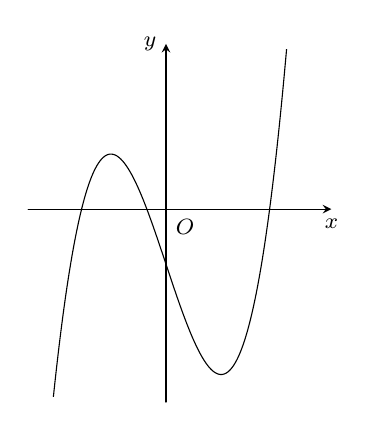
\begin{tikzpicture}[scale=0.7, font=\footnotesize, line join=round, line cap=round,>=stealth]
			\def\a{1} \def\b{0} \def\c{-3} \def\d{-1} % Hệ số
			\def\xmin{-2.5} \def\xmax{3}
			\def\ymin{-3.5} \def\ymax{3} 
			\draw[->] (\xmin,0)--(\xmax,0) node [below]{$x$};
			\draw[->] (0,\ymin)--(0,\ymax) node [left]{$y$};
			\node at (0,0) [below right]{$O$};
			\clip (\xmin+0.1,\ymin+0.1) rectangle (\xmax-0.1,\ymax-0.1);
			\draw[smooth,samples=300] plot(\x,{\a*(\x)^3+\b*(\x)^2+\c*(\x)+\d});
	\end{tikzpicture}}
	\loigiai{
		Đồ thị đã cho là đồ thị hàm số $y=x^3-3x-1$.}
\end{ex}
\begin{ex}%[2D1B5-1]%Câu 42.
	[Mã 101-2022]
	Hàm số nào dưới đây có bảng biến thiên như sau?
	\begin{center}
		
\begin{tikzpicture}
			\tkzTabInit[espcl=2.5,lgt=1.5,nocadre]
			{$x$/0.7,$y'$/0.7,$y$/2.1}
			{$-\infty$,$-1$,$1$,$+\infty$}
			\tkzTabLine{,+,0,-,0,+,}
			\tkzTabVar{-/$-\infty$,+/$2$,-/$-2$,+/$+\infty$}
		\end{tikzpicture}
	\end{center}
	\choice
	{$y=x^4-2x^2$}
	{$y=-x^3+3x$}
	{$y=-x^4+2x^2$}
	{\True $y=x^3-3x$}
	\loigiai{
		Từ bảng biến thiên ta nhận thấy hàm số có hai điểm cực trị và đồng biến trên khoảng $(1;+\infty)$. Do đó hàm số là hàm đa thức bậc ba có hệ số $a>0$. }
\end{ex}
\begin{ex}%[2D1B5-1]%Câu 43.
	[Mã 102 - 2022] Hàm số nào dưới đây có bảng biến thiên như sau?
	\begin{center}
		
\begin{tikzpicture}
			\tkzTabInit[espcl=2.5,lgt=1.5,nocadre]
			{$x$/0.7,$y'$/0.7,$y$/2.1}
			{$-\infty$,$-1$,$1$,$+\infty$}
			\tkzTabLine{,+,0,-,0,+,}
			\tkzTabVar{-/$-\infty$,+/$2$,-/$-2$,+/$+\infty$}
		\end{tikzpicture}
	\end{center}
	\choice
	{$y=-x^3+3x$}
	{\True $y=x^3-3x$}
	{$y=-x^4+2x^2$}
	{$y=x^4-2x^2$}
	\loigiai{
		Từ đồ thị ta có đây là đồ thị hàm số bậc $3$ với hệ số $a>0$.}
\end{ex}
\begin{ex}%[2D1B5-1]%Câu 44.
	[Mã 103 - 2022] Hàm số nào dưới đây có bảng biến thiên như sau
	\begin{center}
		
\begin{tikzpicture}
			\tkzTabInit[espcl=2.5,lgt=1.5,nocadre]
			{$x$/0.7,$y'$/0.7,$y$/2.1}
			{$-\infty$,$-1$,$1$,$+\infty$}
			\tkzTabLine{,-,0,+,0,-,}
			\tkzTabVar{+/$+\infty$,-/$-2$,+/$2$,-/$-\infty$}
		\end{tikzpicture}
	\end{center}
	\choice
	{$y=x^3-3x$}
	{\True$y=-x^3+3x$}
	{$y=x^2-2x$}
	{$y=-x^2+2x$}
	\loigiai{
		Dựa vào bảng biến thiên ta nhận thấy:\\
		Đây là hàm $y=ax^3+bx^2+cx+d(a\neq 0)$.\\
		$\lim\limits_{x\to+\infty} y=-\infty\Rightarrow a<0$.\\
		Do đó hàm số thỏa mãn là $y=-x^3+3x$.}
\end{ex}
\begin{ex}%[2D1B5-1]%Câu 45.
	[Mã 104-2022] Hàm số nào dưới đây có bảng biến thiên như sau?
	\begin{center}
		
\begin{tikzpicture}
			\tkzTabInit[espcl=2.5,lgt=1.5,nocadre]
			{$x$/0.7,$y'$/0.7,$y$/2.1}
			{$-\infty$,$-1$,$1$,$+\infty$}
			\tkzTabLine{,-,0,+,0,-,}
			\tkzTabVar{+/$+\infty$,-/$-2$,+/$2$,-/$-\infty$}
		\end{tikzpicture}
	\end{center}
	\choice
	{$y=x^3-3x$}
	{$y=x^2-2x$}
	{\True $y=-x^3+3x$}
	{$y=-x^2+2x$}	
	\loigiai{
		Dựa vào bảng biến thiên trên, ta nhận thấy đây là hàm số bậc ba có dạng $y=ax^3+bx^2+cx+d$ với $a\neq 0$.\\
		Mà $\lim\limits_{x\to+\infty}\left(ax^3+bx^2+cx+d\right)=-\infty\Rightarrow a<0$.\\
		Do đó có duy nhất hàm số $y=-x^3+3x$ thoả mãn.}
\end{ex}
\Closesolutionfile{ans}
\indapan{10}{ans/CD5/Muc_5_6}